\documentclass{article}
\title{COMS W4115
	Final}
\author{Programming Languages and Translators\medskip\\
	Xijiao Li (xl2950)}
\usepackage{listings}
\usepackage{amsmath}
\usepackage[utf8]{inputenc}
\usepackage{listings}
\usepackage{color}
\usepackage{setspace}
\usepackage{enumitem}
\usepackage{graphicx}
\usepackage{dirtytalk}
\usepackage{tikz}
\usetikzlibrary{automata, positioning, arrows}
\usepackage{booktabs} % For prettier tables

\renewcommand{\baselinestretch}{1.1} 


\definecolor{dkgreen}{rgb}{0,0.6,0}
\definecolor{gray}{rgb}{0.5,0.5,0.5}
\definecolor{mauve}{rgb}{0.58,0,0.82}
\def\code#1{\texttt{#1}}

\lstset{
	%language=Python,
	aboveskip=3mm,
	belowskip=3mm,
	showstringspaces=false,
	columns=flexible,
	basicstyle={\small\ttfamily},
	numbers=none,
	numberstyle=\tiny\color{gray},
	commentstyle=\color{dkgreen},
	stringstyle=\color{mauve},
	breaklines=true,
	breakatwhitespace=true,
	tabsize=3,
	mathescape
}

\begin{document}
	\tikzset{
		->, % makes the edges directed
		>=stealth, % makes the arrow heads bold
		node distance=2.5cm, % specifies the minimum distance between two nodes. Change if necessary.
		every state/.style={thick, fill=gray!10}, % sets the properties for each ’state’ node
		initial text=$ $, % sets the text that appears on the start arrow
	}
	\pagenumbering{gobble}
	\maketitle
	
	\newpage
	\pagenumbering{arabic}
	\subsection*{Problem 20}
	\subsubsection*{1.}
	keyword: $time~|~return$ \\
	identifier: $[a-z][a-z 0-9]^*$\\
	time: $[0-9]^+$\\
	
	\subsubsection*{2.}
	Terminals:
	\begin{table}[h!]
			\begin{tabular}{ |c|c|} 
				\toprule
				$=$ & Assignment Operator\\
				$+$ & Binary Operator\\
				$=$ & Binary Operator\\
				id &  identifier\\
				t &  time\\
				$,$ &  colon\\
				$;$ &  semicolon\\
				$\{$ &  start of block/scope\\
				$\}$ &  end of block/scope\\
				$return$ &  keyword $return$\\
				$time$ &  keyword $time$\\
				\bottomrule
			\end{tabular}
	\end{table}
	
	\noindent Non-Terminals:\\
	$S$: statement\\
	$D$: definition\\
	$B$: block\\
	$P$: parameter \\
	$E$: expression \\
	$L$: literals \\
	$R$: return statement \\
	
	\noindent Start symbol: $S$\\
	
	\noindent Production Rules:	
	\begin{enumerate}[topsep=2pt,itemsep=3pt,parsep=0pt,partopsep=0pt]
		\item $S \rightarrow SS$
		\item $S \rightarrow DB$
		\item $D \rightarrow \text{id}(P)$
		\item $P \rightarrow P,P$
		\item $P \rightarrow time~\text{id}$
		\item $B \rightarrow \{ ER \}$
		\item $E \rightarrow EE$
		\item $E \rightarrow P = L; $
		\item $E \rightarrow \text{id} = L; $
		\item $L \rightarrow L+L$
		\item $L \rightarrow L-L$
		\item $L \rightarrow \text{id}$
		\item $L \rightarrow t$
		\item $R \rightarrow return~\text{id}$
	\end{enumerate}
	
	
	\subsubsection*{3.}
\begin{verbatim}
	test(time t1, time t2){
	   time t3 = t1 + t2;
	   return t3;
	}
\end{verbatim}
	

	\subsubsection*{4.}
	\begin{center}
		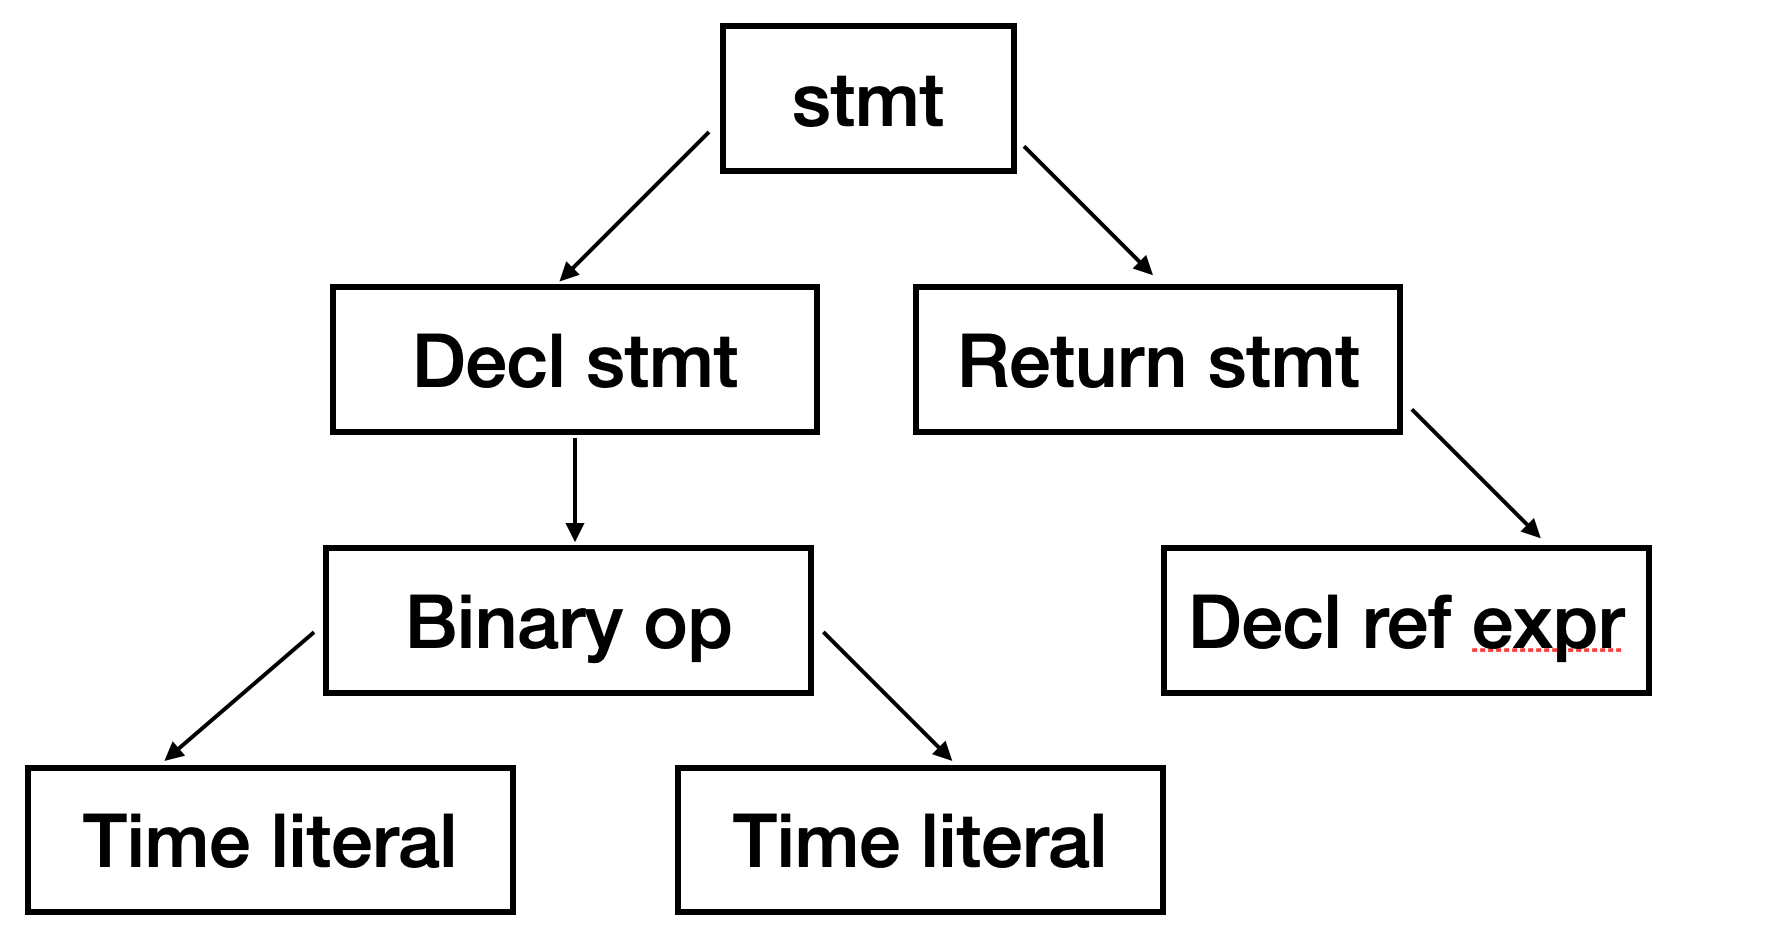
\includegraphics[width=0.6\textwidth]{ast}
	\end{center}

	\subsubsection*{5.}
	\begin{verbatim}
		addi  $sp, $sp, -8
		sw    $a, 4($sp)
		sw    $r, 0($sp)
		add   $a, $a, $r
		j     $a
		nop
		
	\end{verbatim}




	
\end{document}